\documentclass{beamer}
 
\usepackage[utf8]{inputenc}
 \usetheme{Boadilla}
\usepackage{graphicx}
\usepackage{rotating}
\usepackage{ragged2e}
\title{Dynamic Cash Management Models with Loans}
 
%Information to be included in the title page:

\author{Zimian Zhang}


\institute{Lancaster University}

\date{\today}
 
 
 
\begin{document}
\renewcommand{\raggedright}{\leftskip=0pt \rightskip=0pt plus 0cm}
 
\frame{\titlepage}
%table page
\begin{frame}
\frametitle{Outline}
\label{contents}
\tableofcontents
\end{frame}
%!!!!!!!!!!!!!
 
%the FIRST page
%********************************************************************************************************************************************************************************************************************************************************************************************************************************************************************************************
\section{Introduction}

\begin{frame}
\label{cashproblem}
\frametitle{\hyperlink{intro}{What is cash management problem?}}

\begin{columns}
\column{0.4\textwidth}
\begin{itemize}
\item<1-> Consider yourself as a manager of a company.
\item<2-> You want to allocate your money into different assets, such as:
\begin{itemize}
\item<3-> Manufacturing Equipment;
\item<4-> Inventory;
\item<5-> Portfolio;
\item<6-> Loan;
\item<7> Cash;
\end{itemize}
\end{itemize}
\column{0.6\textwidth}
\includegraphics<2>[scale = 0.45]{cp1}
\includegraphics<3>[scale = 0.45]{cp2}
\includegraphics<4>[scale = 0.45]{cp3}
\includegraphics<5>[scale = 0.45]{cp4}
\includegraphics<6>[scale = 0.45]{cp5}
\includegraphics<7>[scale = 0.45]{cp6}
\end{columns}
\end{frame}

\begin{frame}
\frametitle{\hyperlink{intro}{What is cash?}}
\begin{columns}
\column{0.4\textwidth}
\begin{sideways}
\centering
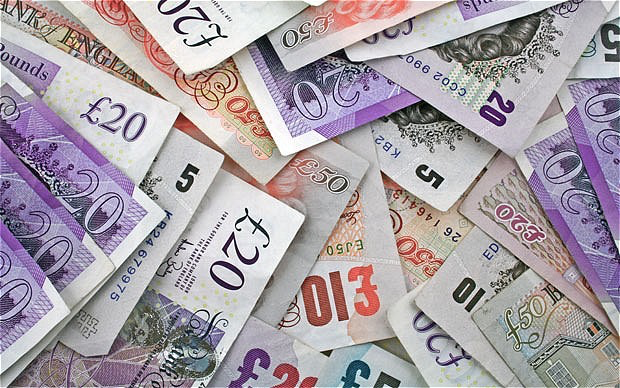
\includegraphics[scale = 0.25]{cash}
\end{sideways}
\column{0.6\textwidth}
In cash management problem, cash is considered as an asset with most liquidity and low/none profitability.

\begin{itemize}
\item<2-> \textbf{High Liquidity}: Cash can be `sold' for any other asset without loss of value or wait for a suitable buyer of cash.
\item<3-> \textbf{Low/none Profitability}: Cash can be considered as an investment with very low, if there is any, return.
\item<4>\textbf{Why cash?}: Cash demand: Salaries, Utility bills, Shareholder redemption, etc.
\end{itemize}

\end{columns}
\end{frame}


\begin{frame}

\begin{block}{Cash Management Problem}
What is the strategy of allocating money to this asset `cash'?
\end{block}

\end{frame}



%!!!!!!!!!!!!!
\begin{frame}
\label{cashproblem}
\frametitle{\hyperlink{intro}{What is cash management problem?}}
\begin{columns}
\column{0.4\textwidth}
\begin{itemize}
\item<3->With insufficient cash holding level, a company might expose to the risk of cash deficit, which might cause a great amount of penalty.
\item<4->On the other hand, a high cash-holding level normally means the inefficient use of firm's resource, which would constrain firm's future profitability.
\end{itemize}
\column{0.6\textwidth}
\includegraphics<2->[scale = 0.27]{holdingCost.png}
\end{columns}
\end{frame}



\begin{frame}
\frametitle{Models from literature}

\begin{small}
\begin{itemize}

\item<2-> A basic cash management model 

\includegraphics<3>[scale = 0.35]{basicModel.png}
\end{itemize}

\begin{itemize}
\item<4-> A CM model in a randomly varying environment  (Hinderer, Waldmann, 2001)

\includegraphics<5>[scale = 0.25]{EnvMod.png}
\end{itemize}

\begin{itemize}
\item<6-> A CM model with two accounts (Bensoussan, Chutani, and Sethi, 2009)

\includegraphics<7>[scale = 0.25]{otherTwoAsset.png}
\end{itemize}

\begin{itemize}
\item<8-> A CM model with different cash demand (Nascimento, and Powell, 2010)

\includegraphics<9>[scale = 0.25]{mutualFund.png}
\end{itemize}


\begin{itemize}
\item<10-> A CM model with different cash sources (Sato, and Sawaki, 2009)

\includegraphics<11>[scale = 0.25]{twoSource.png}

\end{itemize}
\end{small}



\end{frame}


\begin{frame}
\frametitle{Motivation}
\begin{itemize}
\item<2->Most literature considers cash flows as an exogenous variable.

\item<3->We consider cash flows as a superposition of the exogenous variable and endogenous variable.
\item<4->We consider the scenario where the company can finance itself by taking loans.


\end{itemize}


\end{frame}


\begin{frame}
\frametitle{Cash management model with loans}
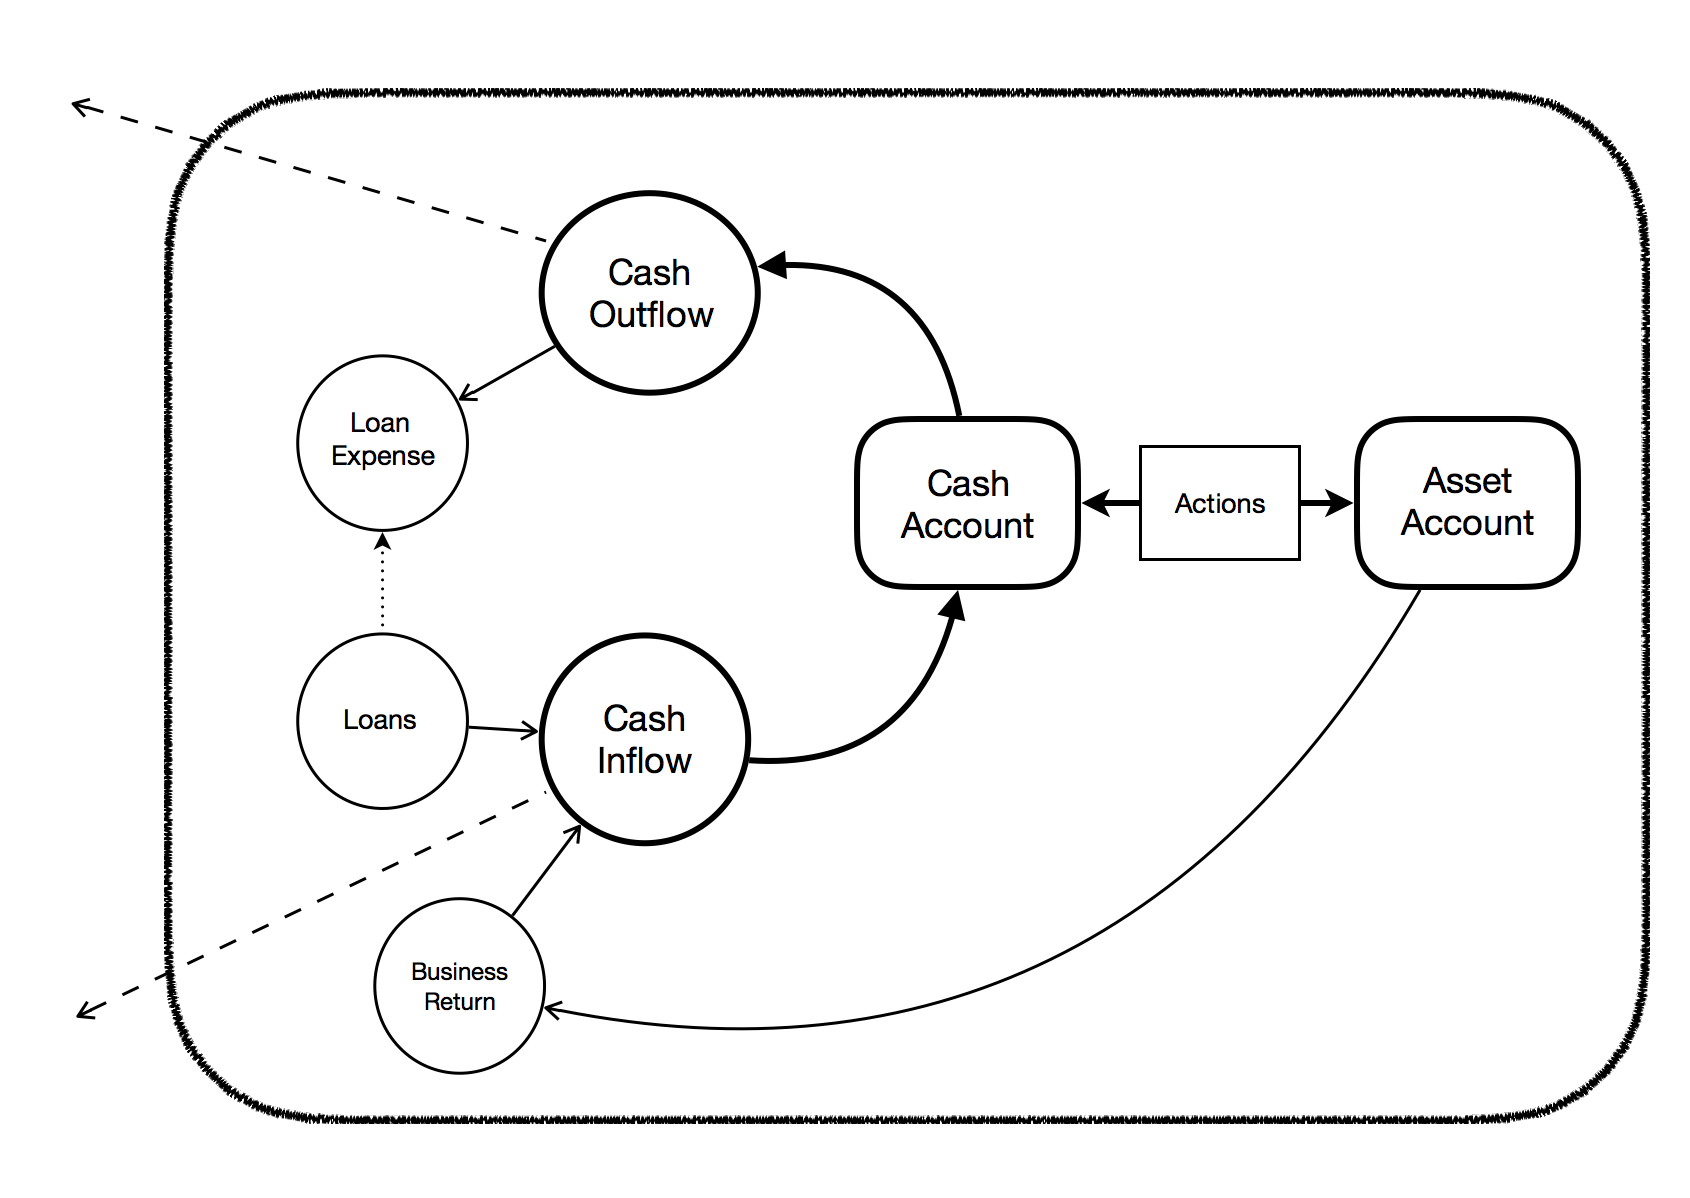
\includegraphics[scale = 0.4]{loan.png}

\end{frame}

\section{A two-assets cash management model}

\begin{frame}
\frametitle{The two assets CM model}
\begin{itemize}

\item Objective function: Maximising net profits $$\max \sum^\infty _{t = 0}\gamma^t  \{ rr \cdot y_t - D_t - \Gamma_t - SC_t \}.$$
\item A partially fixed and partially proportional transaction cost function$$\Gamma(a) =  (K_c + k_c a) \cdot 1_{\{ a < 0\}} + (K_a +k_aa)\cdot 1_{\{a>0\}}$$
\item Cash shortage cost: $$SC(x_t) = 1_{\{ x_t < 0\}} \cdot \{SP+\Gamma(|x_t|) \}$$
\item Options of declaring bankruptcy
\item Loans unavailable.
\end{itemize}
\end{frame}





\begin{frame}
\frametitle{States Transition}
\begin{itemize}
\item Markov Decision Process
\begin{columns}
\column{0.3\textwidth}


\begin{itemize}

\item<1-> Discrete State:

\item<2-> Cash inflow: 



\item<3-> Decision:

\item<4-> Cash outflow:

\item<5-> Cash shortage?

\end{itemize}


\column{0.7\textwidth}
\only<1> {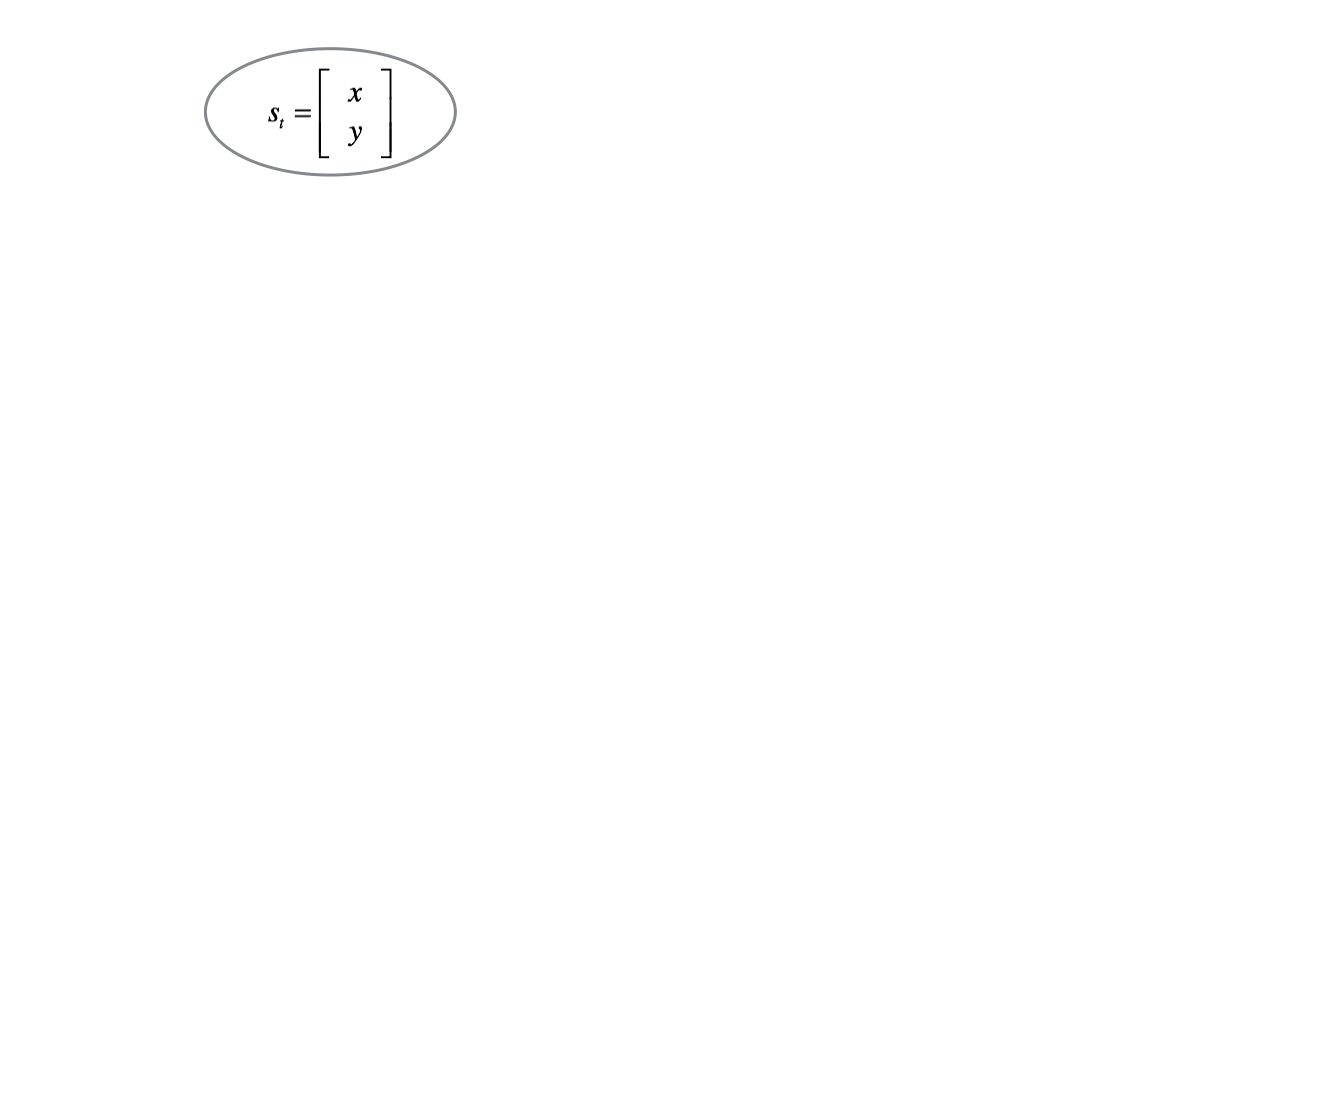
\includegraphics[scale=0.35]{mdp1}}


\only<2> {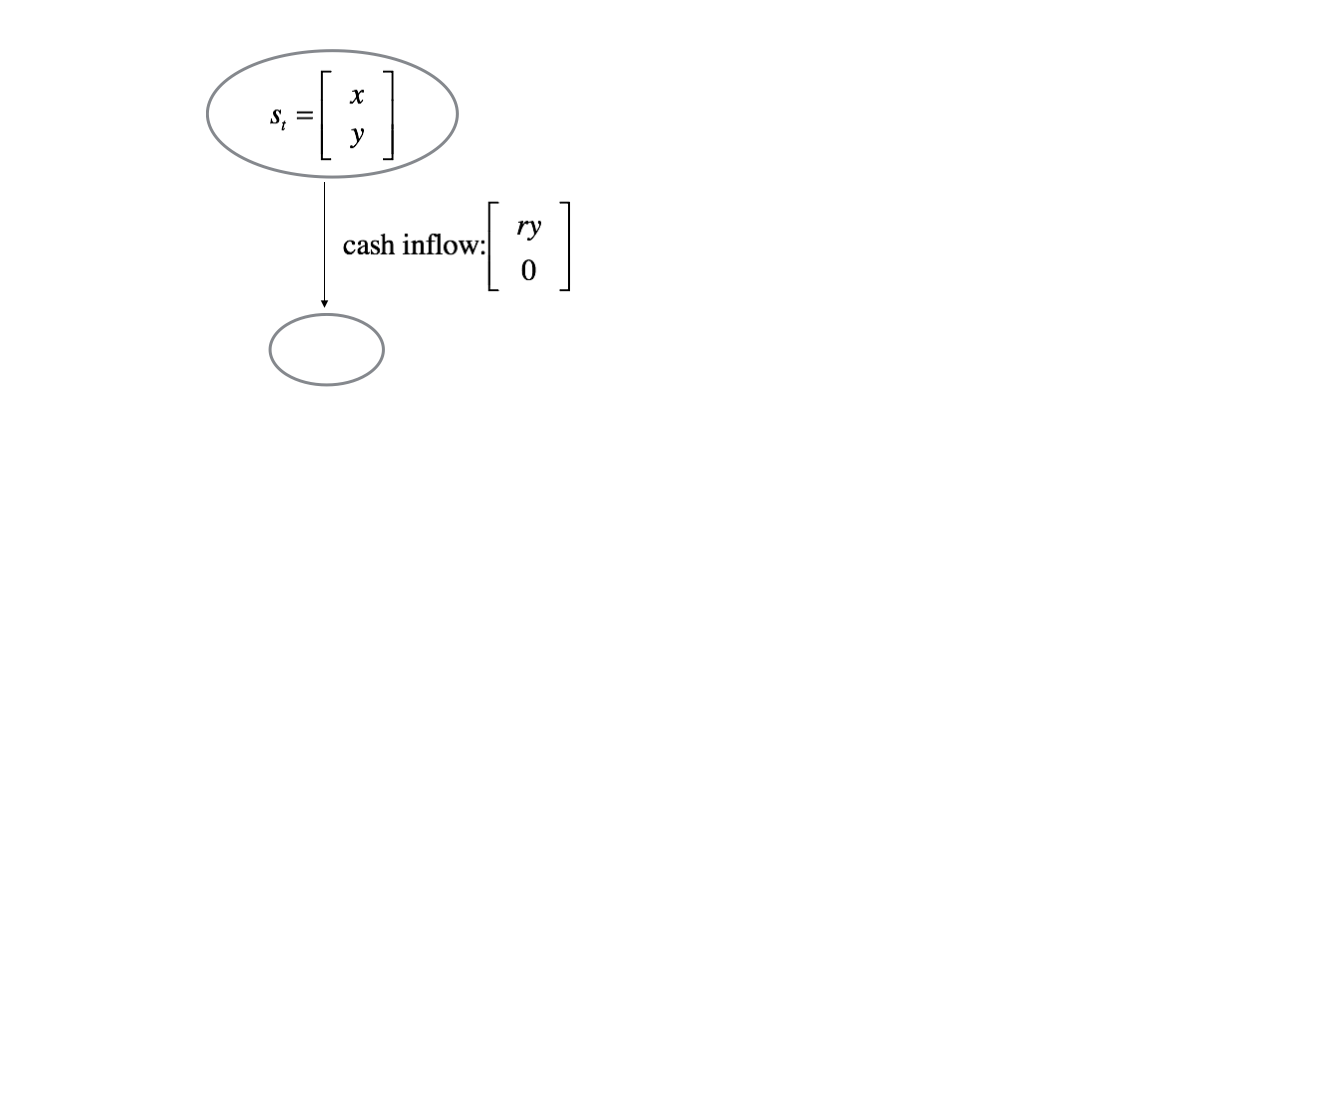
\includegraphics[scale=0.35]{mdp2}}

\only<3> {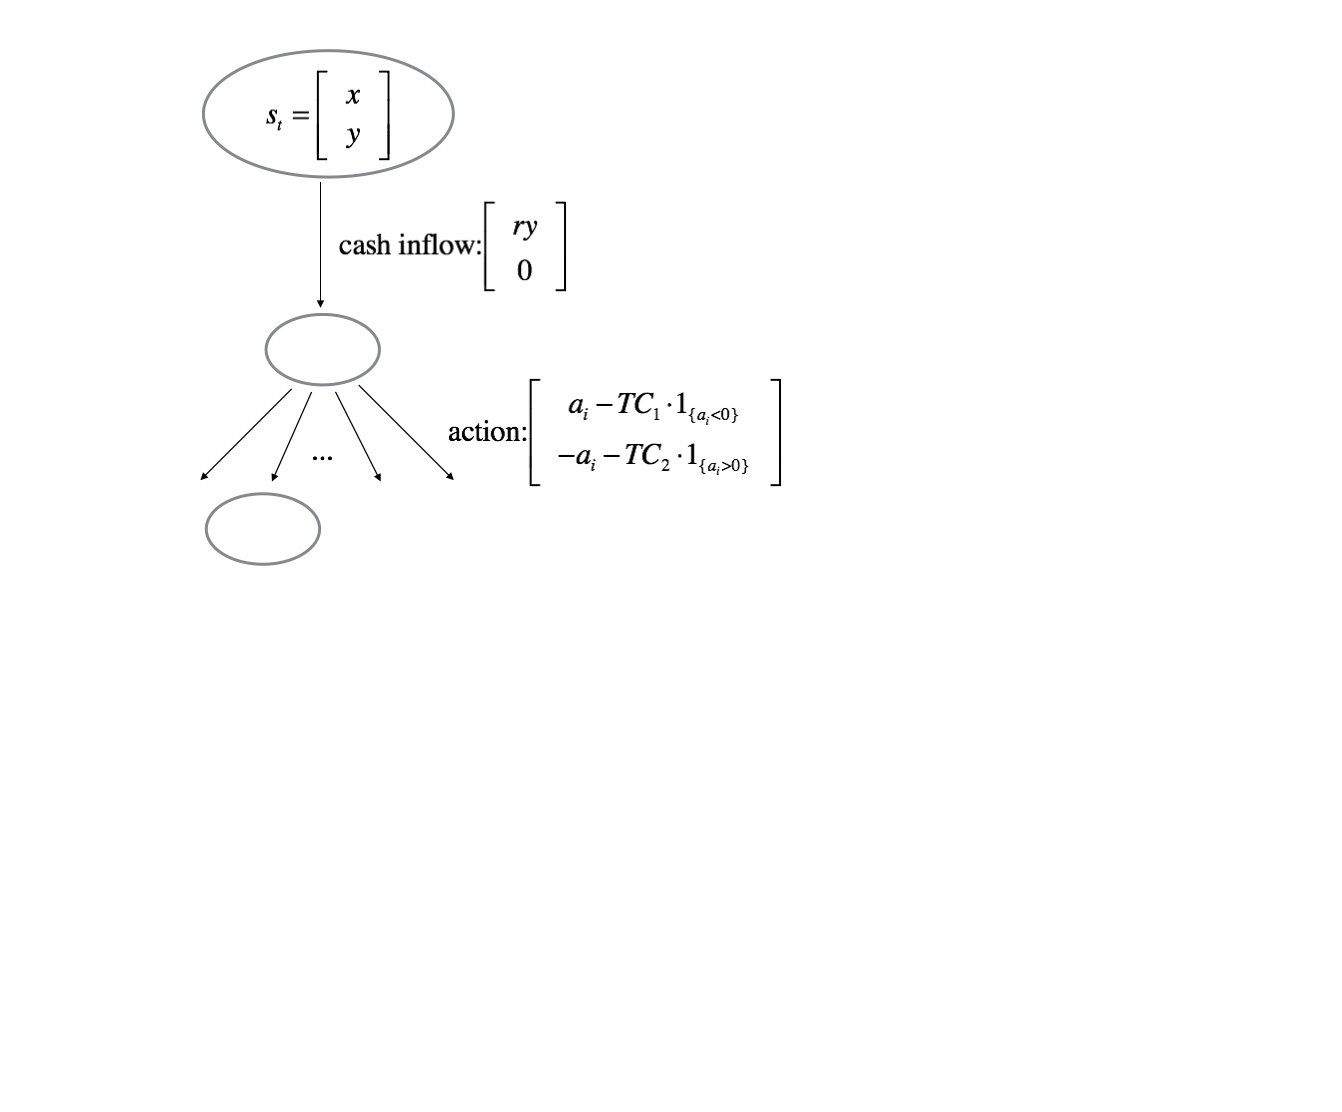
\includegraphics[scale=0.35]{mdp3}}

\only<4> {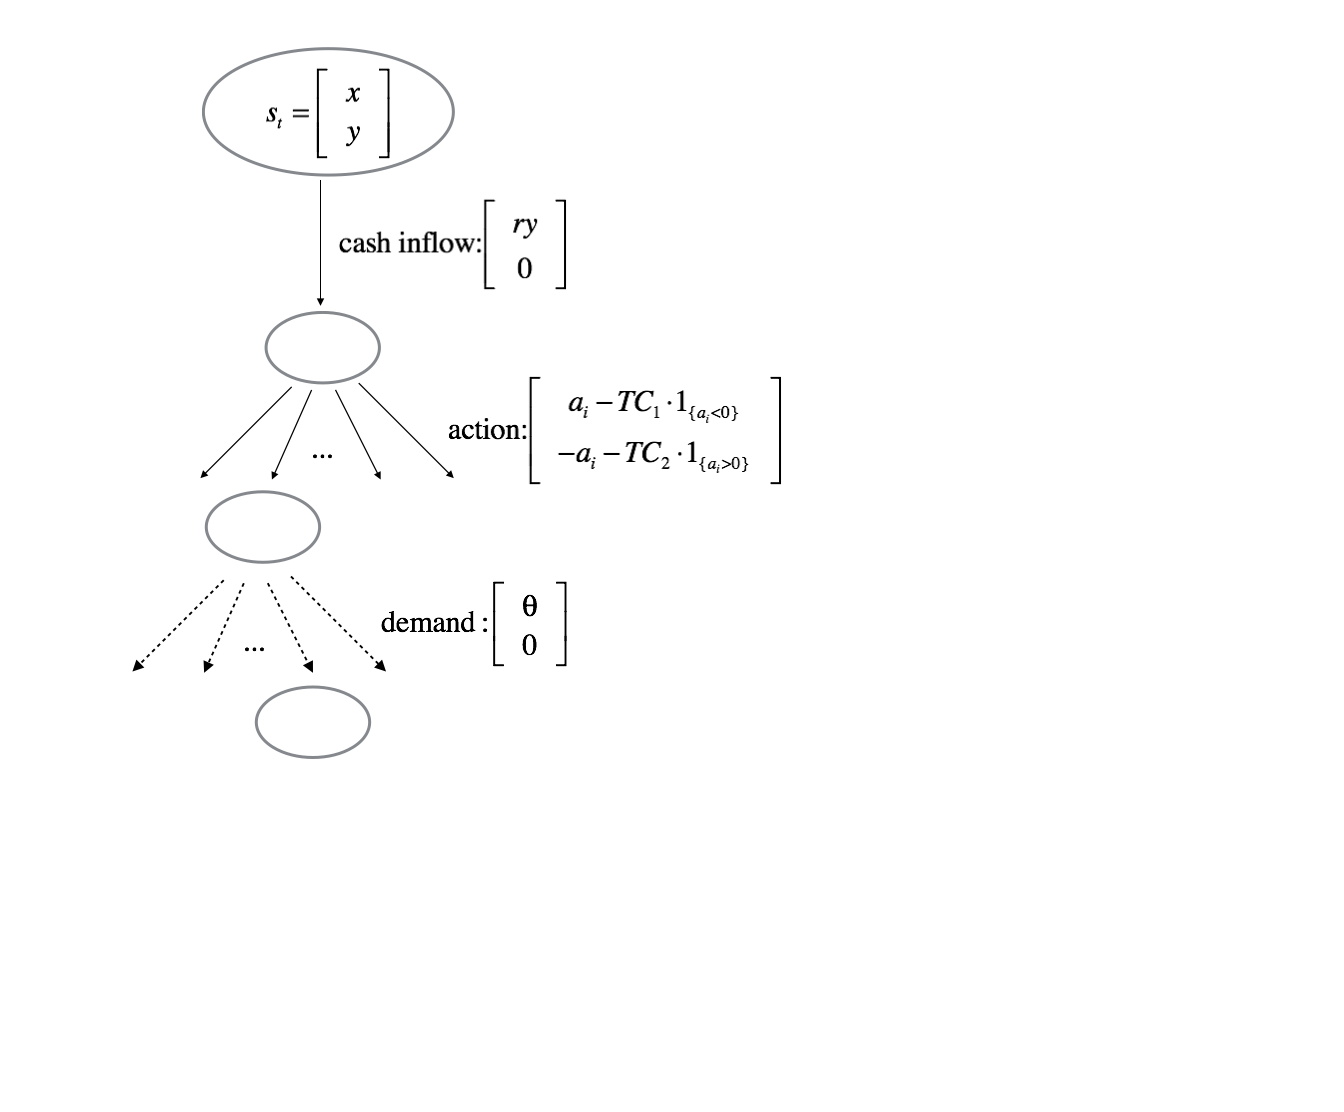
\includegraphics[scale=0.35]{mdp4}}

\only<5> {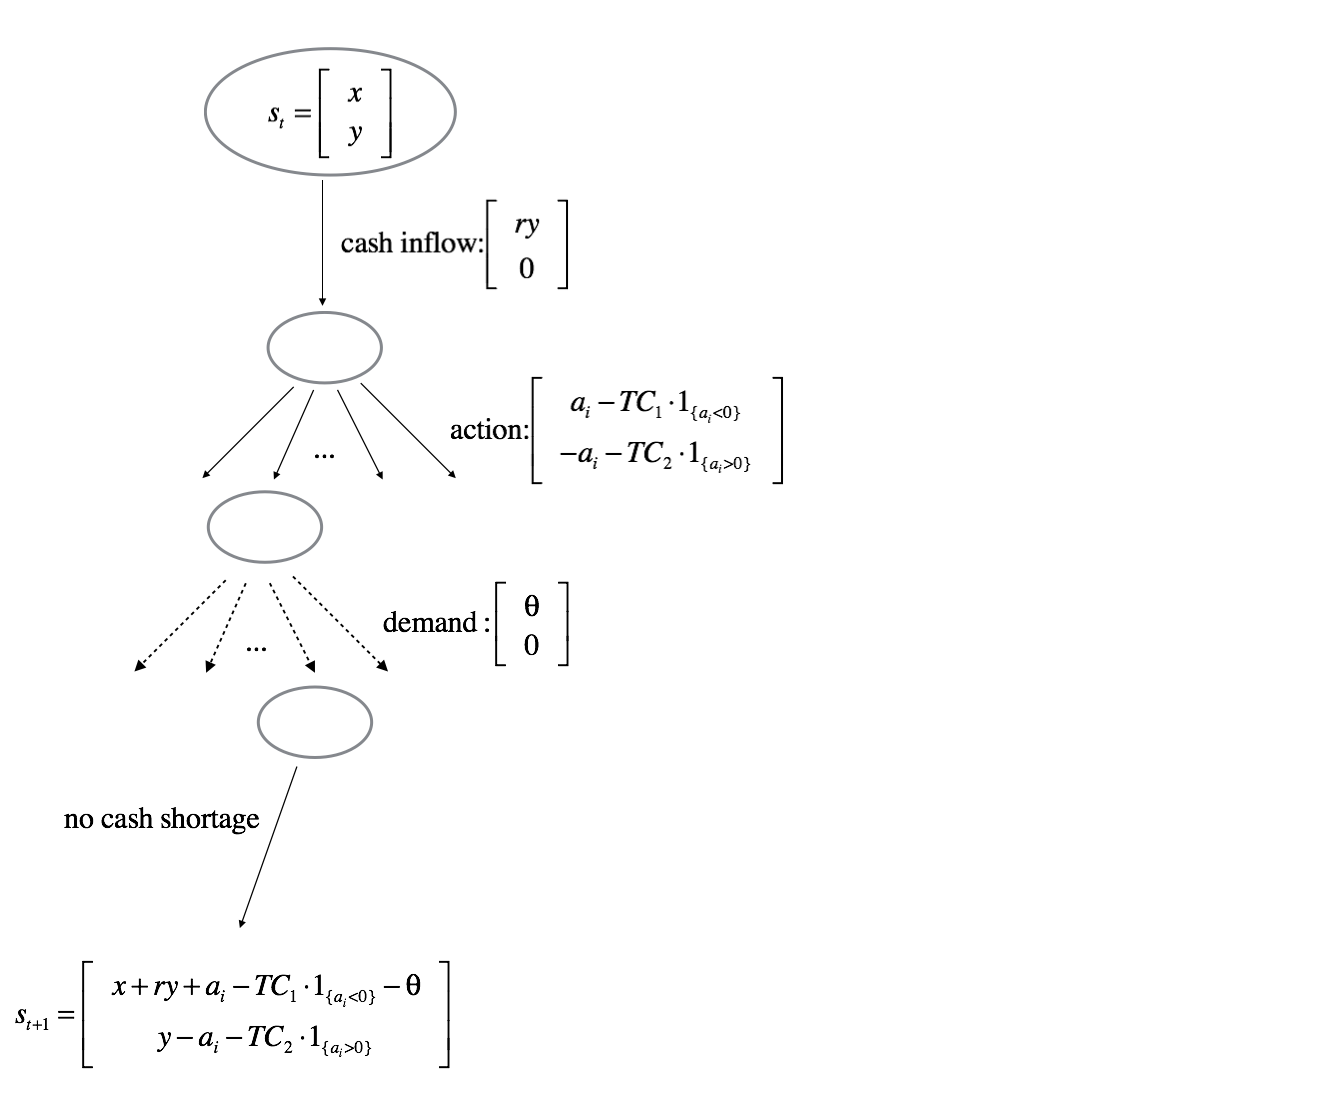
\includegraphics[scale=0.35]{mdp5}}

\only<6> {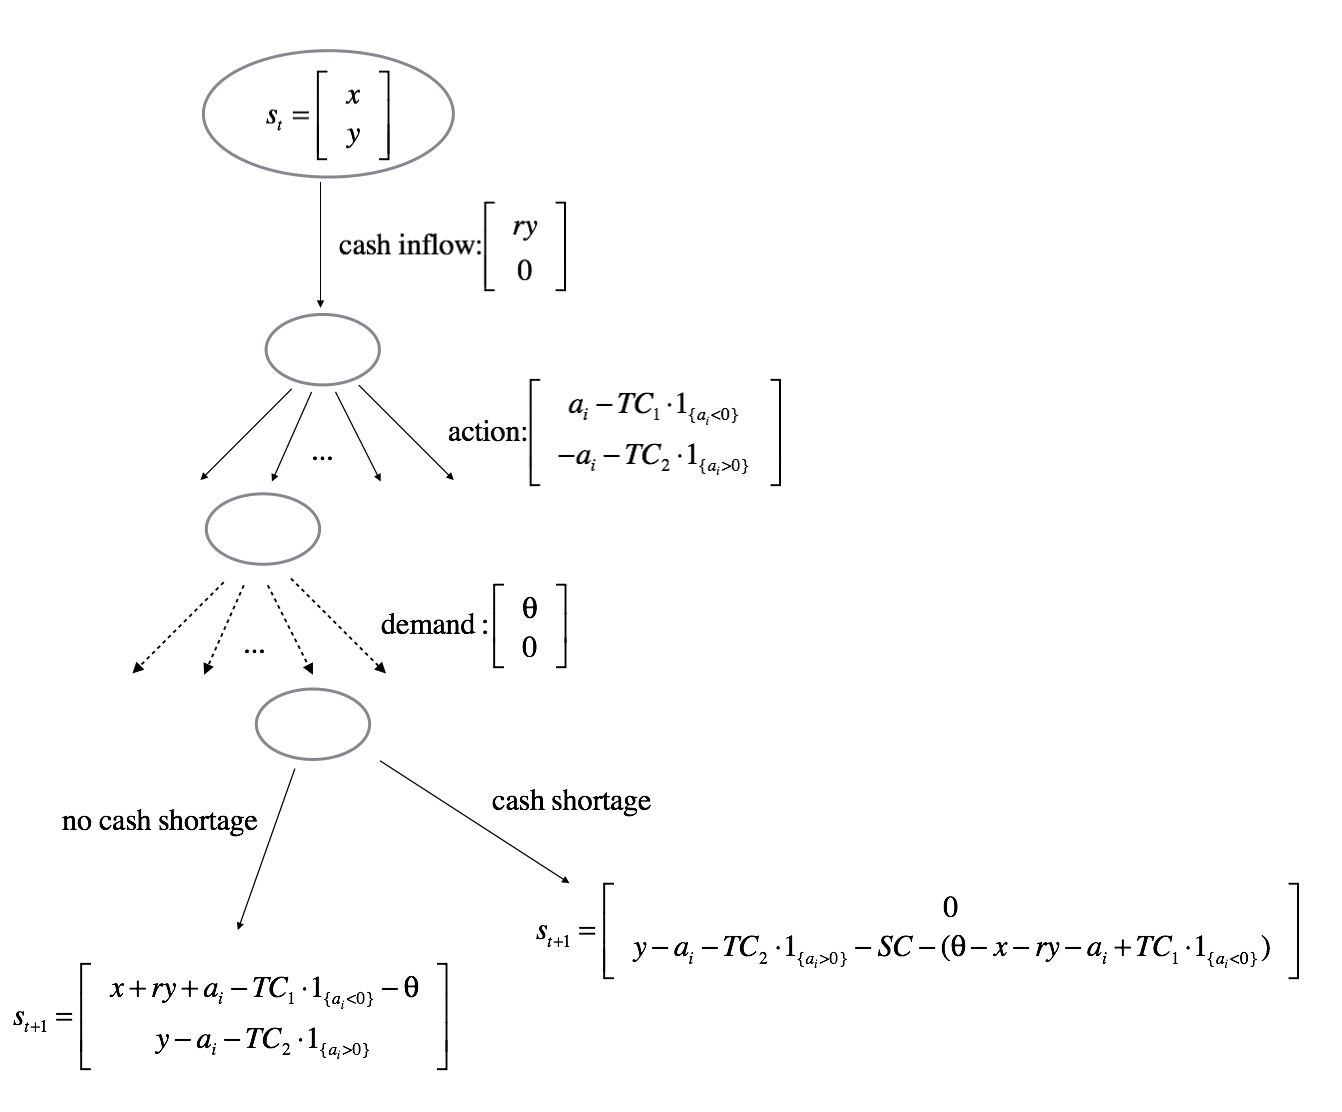
\includegraphics[scale=0.35]{mdp6}}


\end{columns}
\end{itemize}
\end{frame}












\begin{frame}
\frametitle{An optimal solution of the two-asset CM model}
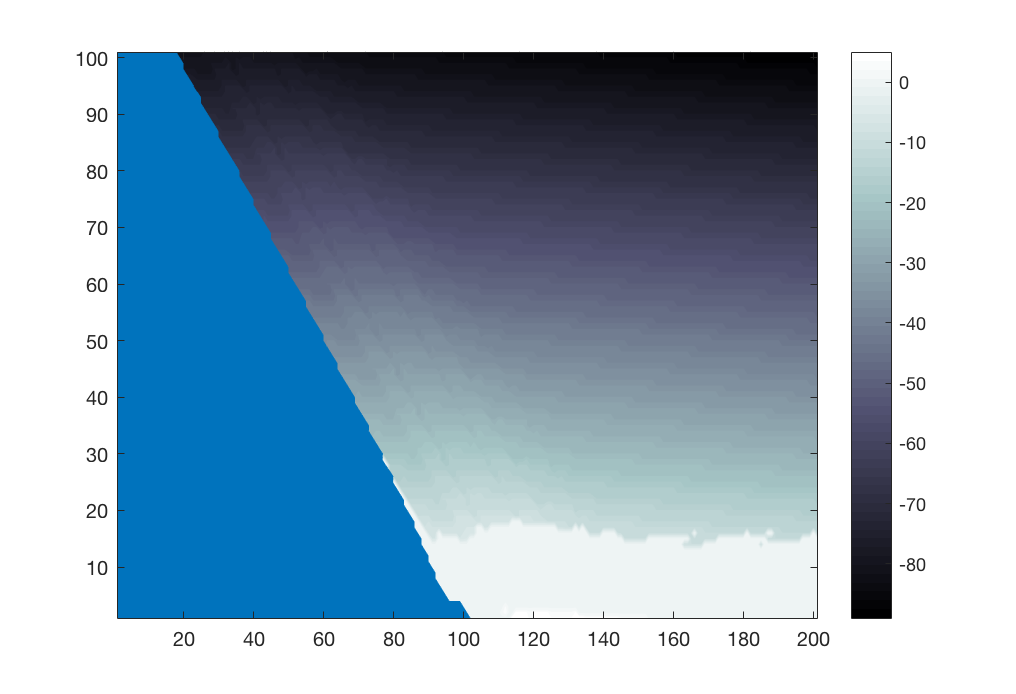
\includegraphics[scale = 0.25]{new.png}
\end{frame}

\begin{frame}
\frametitle{Simulation of the strategy}
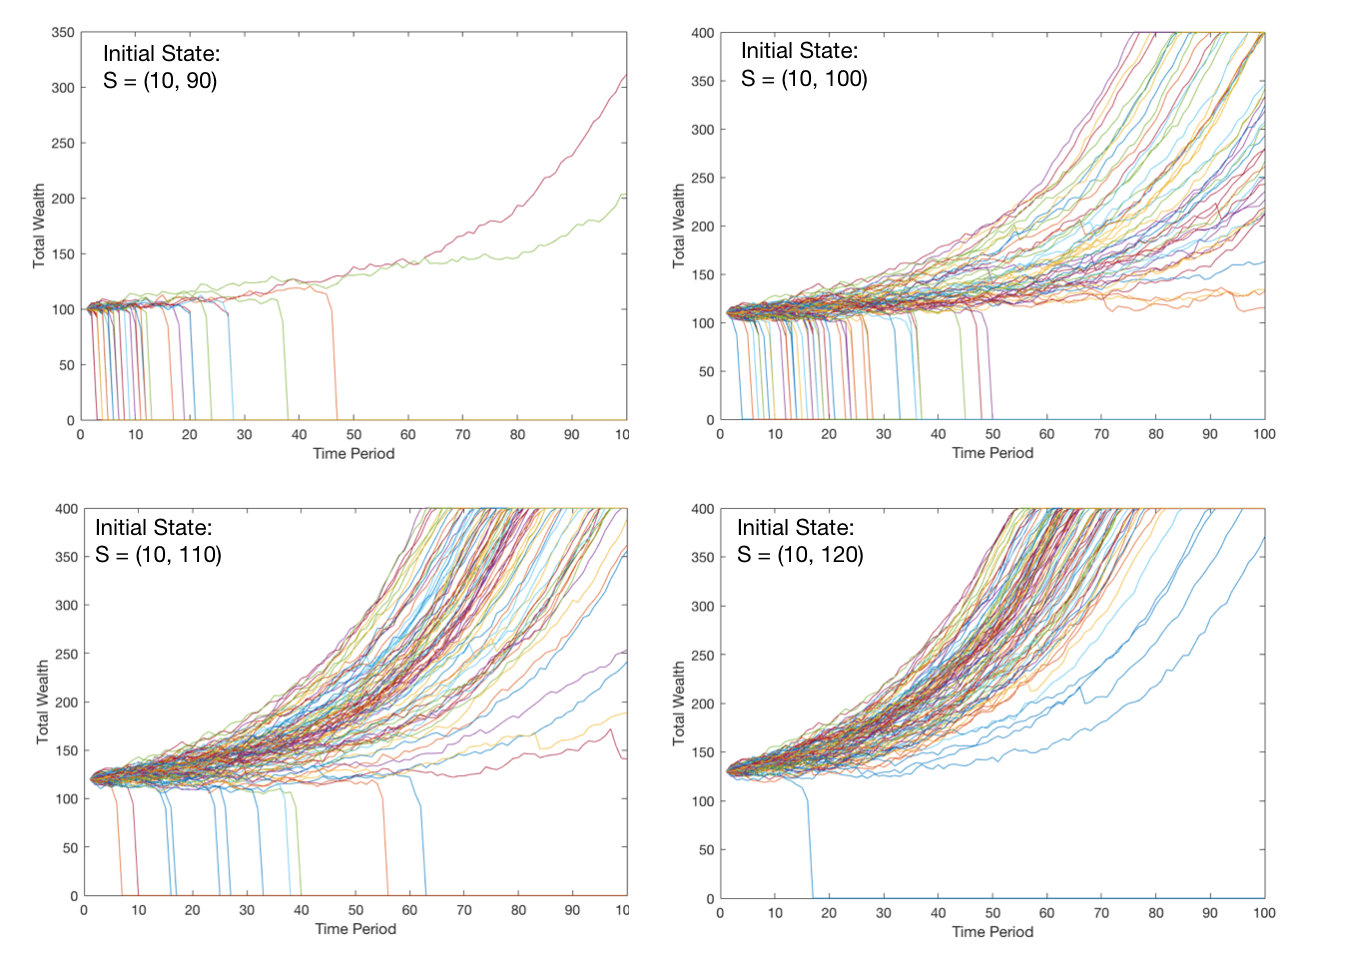
\includegraphics[scale = 0.4]{simu.png}
\end{frame}

\begin{frame}
\frametitle{Probability of going bankrupt}
\begin{itemize}
\item At stage 0 (the last period of time planning horizon), any state $S_{x, y}$ with $y \neq 0$ has value (probability of going bankrupt) equal to 0 and any state $S_{x, y}$ with $y = 0$ has value (probability of going bankrupt) equal to1.
\item for any stage $k: k \geq 1$

\[
\begin{split}
V_{[x,y]}^{k} =& \sum P\left\{\left.S_{(0,0)}:W(S_{x,y}) = S_{(0,0)}\right|a = A^*(S_{x,y})\right\} 
\\ 
+ & \sum P\left\{ \left. S_{x',y'}:W(S_{x,y}) = S_{x',y'} \right| a = A^* (S_{x,y})\right\}  V_{[x',y']}^{k-1}
\end{split}
\]
where $V_{[x,y]}^{k} $ is the probability that the company will eventually going bankrupt if it is in state $S_{x,y}$ at stage $k$
\end{itemize}
\end{frame}

\section{Cash management model with loan options}
\begin{frame}
\frametitle{Cash management with loan options}
\begin{itemize}
\item State: $S_{x,y,z}$ where $x$ and $y$ represent the current cash and asset level and $z$ represent the remaining times of loan repayment.
\item Loan Repayment $LP$: let $L$ be the loan size, $lr$ be the loan rate and once the manager take the loan, he has to make an equally amount of repayment in following $N$ time periods. Then for each time period, he has to pay $$LP = L \cdot \frac{lr \cdot (1+lr)^N}{(1+lr)^N-1}$$
\item We assume that companies with debt unpaid cannot take more loans.
\item At time $t$, if the manager take the loan, then the cash inflow increases by $L$ amount and its loan state $s$ changes from $0$ to $N$. In the following $N$ time periods, the company's cash demand will increase by LP amount and $z$ value decreases by $1$. 
\end{itemize}
\end{frame}

\begin{frame}
\frametitle{Cash management with loan options}
\begin{itemize}
\item<2-> Limitation: we can formulate this model as a Markov Decision Process problem. But the computation cost will increase dramatically.
\begin{itemize}
\item<3-> State Space: $X \times Y \times Z$
\item<3-> Action Space: $A \times L $
\end{itemize}
\item<4->  Heuristic Method: One-step policy improvement.


\includegraphics<4->[scale=.3]{heuristic.png}

\end{itemize}
\end{frame}

\begin{frame}
\frametitle{Simulation results of one-step policy improvement}
Assume there is only one loan available on the market: $L = 40, lr = 0.03, N = 40$


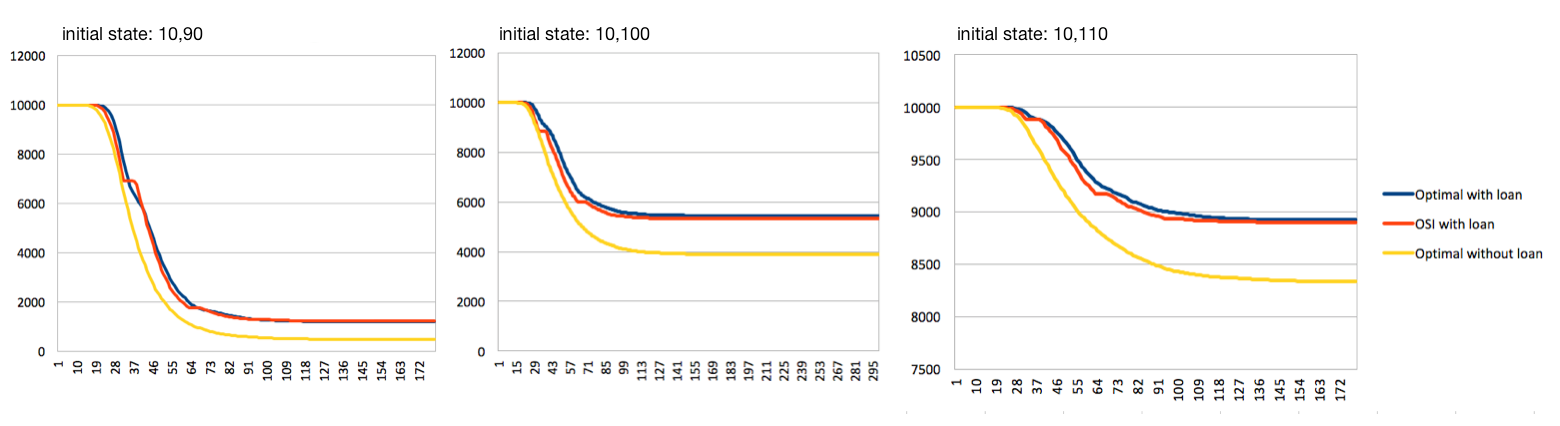
\includegraphics[scale=.22]{oneStep}
\end{frame}




\section{Future Research}
\begin{frame}
\frametitle{Future Research}
\begin{itemize}
\item Multi-loan case: Companies in better states could get a better loan.
\item Environmental factors.
\item Other actions the manager could take while manage the cash, such as taking investment, open a new branch, etc.
\end{itemize}
\includegraphics<4->[scale=.18]{Holistic.png}
\end{frame}




\begin{frame}

\includegraphics[scale=.4]{tky}
\end{frame}

\end{document}